\documentclass[12pt]{article}
\usepackage{ctex}
\usepackage{graphicx}
\usepackage{subfigure}
\usepackage{caption}
\usepackage{float}
\usepackage{physics}
\usepackage{amsmath}
\usepackage{slashed}
\usepackage{geometry}
\geometry{left=2.5cm,right=2.5cm,top=2.5cm,bottom=2.5cm}
\title{Solution to Problem V-2}
\author{Zhang Tingyu $\ $ 35206402}
\graphicspath{{figures/}}

\begin{document}

\maketitle

\section*{(a)}

Trivial.

\section*{(b)}

In this $e^-+e^+\rightarrow\tilde{\mu}^-+\tilde{\mu}^+$, We can write down the 
Feynman rules:
\begin{figure}[H]
    \centering
    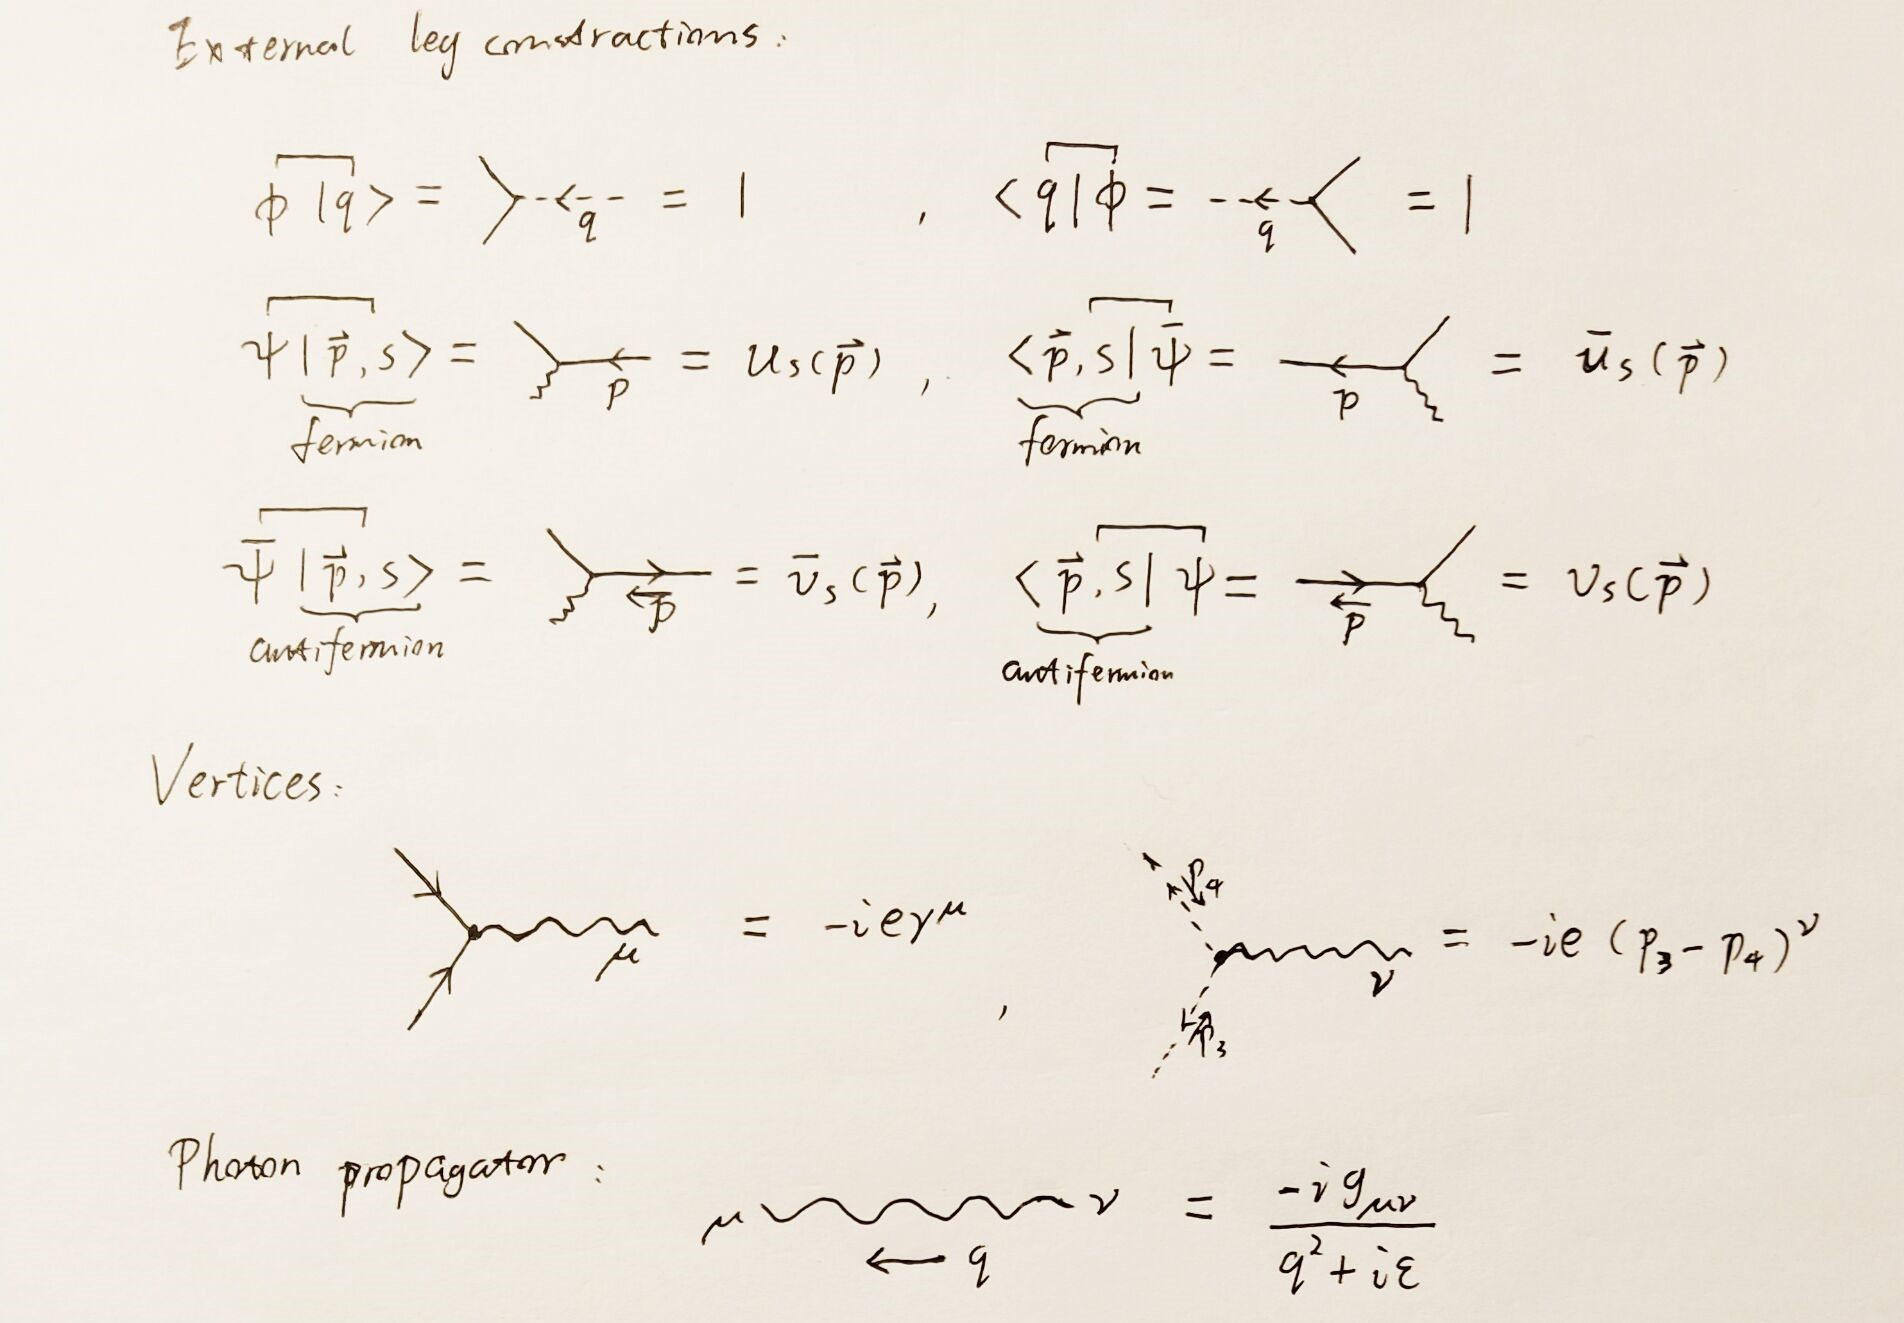
\includegraphics[width=15cm]{1.jpg}
    \caption*{}
    \label{}
\end{figure}
Thus we can write the  scattering amplitude as 
\begin{equation}
    \begin{split}
        &i\mathcal{M}\left(e_{r}^{-}\left(\vec{p}_{1}\right)+e_{s}^{+}\left(
        \vec{p}_{2}\right) \rightarrow \tilde{\mu}^{-}\left(\vec{p}_{3}
        \right)+\tilde{\mu}^{+}\left(\vec{p}_{4}\right)\right)\\
        =&\bar{v}_s(\vec{p}_2)\big(-ieQ_e\gamma^\mu\big)u_r(\vec{p}_1)\frac{-ig_{\mu\nu}}
        {(p_1+p_2)^2+i\epsilon}\big(-ieQ_\mu(p_3-p_4)^\nu\big)\\
        =&\frac{i\left(Q_\mu Q_e e^2\right)}{(p_{1}+p_{2})^{2}+i\epsilon}
        \left(\bar{v}_{s}\left(\vec{p}_{2}\right)\gamma^{\mu} u_{r}\left(\vec{p}_{1}
        \right)\right)\left(p_{3}-p_{4}\right)_{\mu}.
    \end{split}
\end{equation}

\section*{(c)}

In the center of mass frame ($\vec{p}_2=-\vec{p}_1$ and $\vec{p}_4=-\vec{p}_3$), 
the average of $|\mathcal{M}|^2$ can be written as 
\begin{equation}
    \begin{split}
        \frac{1}{4}\sum_{r,s}|\mathcal{M}|^2&=\frac{1}{4}\frac{(Q_\mu Q_e e^2)^2}
        {s^2}[\bar{v}_s(\vec{p}_2)\gamma^\mu u_r(\vec{p}_1)][\bar{u}_r(\vec{p}_1)
        \gamma^\nu v_s(\vec{p}_2)](p_3-p_4)_\mu(p_3-p_4)_\nu\\
        &=\frac{1}{4}\frac{(Q_\mu Q_e e^2)^2}{s^2}\Tr\big[\gamma^\mu(\slashed{p}_1+m_e)
        \gamma^\nu(\slashed{p}_2-m_e)\big](p_3-p_4)_\mu(p_3-p_4)_\nu.
    \end{split}
\end{equation}
Notice that in the center of mass frame, 
\begin{equation*}
    (p_3-p_4)_\mu=\left\{\begin{aligned}
        &0 \qquad\  for\ \mu=0\\
        &2p_{3i}\quad for\ \mu=i\ (i=1,2,3)
    \end{aligned}
    \right.,
\end{equation*}
the equation above can be written as 
\begin{equation}
    \begin{split}
        \frac{1}{4}\sum_{r,s}|\mathcal{M}|^2&=4\frac{(Q_\mu Q_e e^2)^2}{s^2}
        \Big[-m_e^2\delta^{ij}-(p_1\cdot p_2)\delta^{ij}+p_1^{\ i}p_2^{\ j}+
        p_1^{\ j}p_2^{\ i}\Big]p_{3i}p_{3j}\\
        &=4\frac{(Q_\mu Q_e e^2)^2}{s^2}\bigg\{\Big[-m_e^2\delta^{ij}-\Big(\frac{s}{2}
        -m_e^2\Big)\delta^{ij}\Big]p_{3i}p_{3j}-2\big(\vec{p}_1\cdot\vec{p}_3\big)^2
        \bigg\}\\
        &=\frac{(Q_\mu Q_e e^2)^2}{s^2}\bigg[4m_e^2|\vec{p}_3|^2-
        8\big(\vec{p}_1\cdot\vec{p}_3\big)^2+4\Big(\frac{s}{2}-m_e^2\Big)
        |\vec{p}_3|^2\bigg]
    \end{split}
\end{equation} 

\section*{(d)}

In the center of mass frame, $s=(p_1+p_2)^2=4E_{\vec{p}_1}^2$. When the energy of the 
$e^-+e^+$ collision is just high enough for a $\tilde{\mu}^-+\tilde{\mu}^+$ pair 
creation ($|\vec{p}_1|\simeq E_{\vec{p}_1}\simeq M_\mu$), the average of 
$|\mathcal{M}|^2$ can be written as
\begin{equation}
    \begin{split}
        \frac{1}{4}\sum_{r,s}|\mathcal{M}|^2&=\frac{(Q_\mu Q_e e^2)^2}
        {16E_{\vec{p}_1}^4}\Big[4m_e^2|\vec{p}_3|^2-8\big(\vec{p}_1\cdot
        \vec{p}_3\big)^2+4|\vec{p}_3|^2\big(2E_{\vec{p}_1}^2-m_e^2\big)\Big]\\
        &=\frac{(Q_\mu Q_e e^2)^2}{16E_{\vec{p}_1}^4}\Big[8E_{\vec{p}_1}^2
        |\vec{p}_3|^2-8\big(\vec{p}_1\cdot\vec{p}_3\big)^2\Big]\\
        &\simeq\frac{(Q_\mu Q_e e^2)^2}{2}\Bigg[\frac{|\vec{p}_3|^2}{M_\mu^2}
        \Bigg(1-\frac{(\vec{p}_1\cdot\vec{p}_3)^2}{M_\mu^2|\vec{p}_3|}\Bigg)\Bigg]\\
        &\simeq\frac{(Q_\mu Q_e e^2)^2}{2}\Bigg[\frac{|\vec{p}_3|^2}{M_\mu^2}
        \Bigg(1-\frac{(\vec{p}_1\cdot\vec{p}_3)^2}{|\vec{p}_1|^2|\vec{p}_3|^2}\Bigg)\Bigg]\\
        &=\frac{(Q_\mu Q_e e^2)^2}{2}\beta_\mu^2\sin^2\theta
    \end{split}
\end{equation}
where $\beta_\mu:=|\vec{p}_3|/M_\mu$ is the velocity of the produced 
$\tilde{\mu}^\pm$ and $\theta$ is the scttering angle in the center of mass frame.

\section*{(e)}

In the high energy limit, $|\vec{p}_1|\simeq E_{\vec{p}_1}\simeq|\vec{p}_3|$.
\begin{equation}
    \begin{split}
        \frac{1}{4}\sum_{r,s}|\mathcal{M}|^2&=\frac{(Q_\mu Q_e e^2)^2}{16E_{\vec{p}_1}^4}
        \Big[8E_{\vec{p}_1}^2|\vec{p}_3|^2-8\big(\vec{p}_1\cdot\vec{p}_3\big)^2\Big]\\
        &=\frac{(Q_\mu Q_e e^2)^2}{2E_{\vec{p}_1}^4}\Big[E_{\vec{p}_1}^2|\vec{p}_3|^2
        -|\vec{p}_1|^2|\vec{p}_3|^2\cos^2\theta\Big]\\
        &\simeq\frac{(Q_\mu Q_e e^2)^2}{2}\big[1-\cos^2\theta\big]\\
        &=\frac{(Q_\mu Q_e e^2)^2}{2}\sin^2\theta
    \end{split}
\end{equation}

\end{document}